\iffalse
\bibliography{myreference.bib}
\fi

%chapter 3
\chapter{Data Preparation}
\section{Dataset source}
The dataset are acquired from the link provided in this paper\cite{wu2015false}. The original dataset are composed of four contents. 
\begin{figure}[h]\centering 
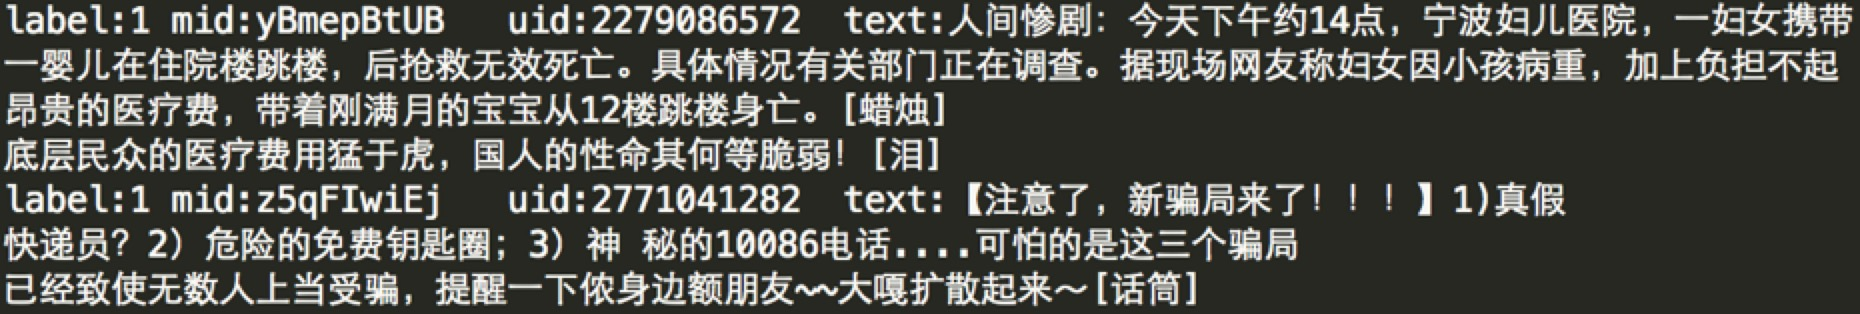
\includegraphics[width=1\textwidth]{originaldata}
\caption{Sample in Original Dataset}\label{fig:originaldataset} \end{figure}

\begin{enumerate} \item mid: The id of individual Weibo \item uid: The id of individual user \item Text \item label: the class of that Weibo, 1 for rumor and 0 for not rumor.
\end{enumerate}

This dataset only contains these four items. Thus we need to crawl more features from Sina Weibo. There are various API provided by Sina Weibo. Since we have the Id of Weibo, we can use it in Java as followed:
\clearpage
\begin{lstlisting}[language=inform]
import weibo4j.Timeline;
import weibo4j.model.Status;
Timeline tm = new Timeline();
Status status = tm.showStatus(id);
\end{lstlisting}
We need the id of Weibo as the input. The data are returned as JSON. The class \textit{Status} has many method to resolve JSON files. Thus it is convenient to acquire various items.
\begin{figure}[h]\centering 
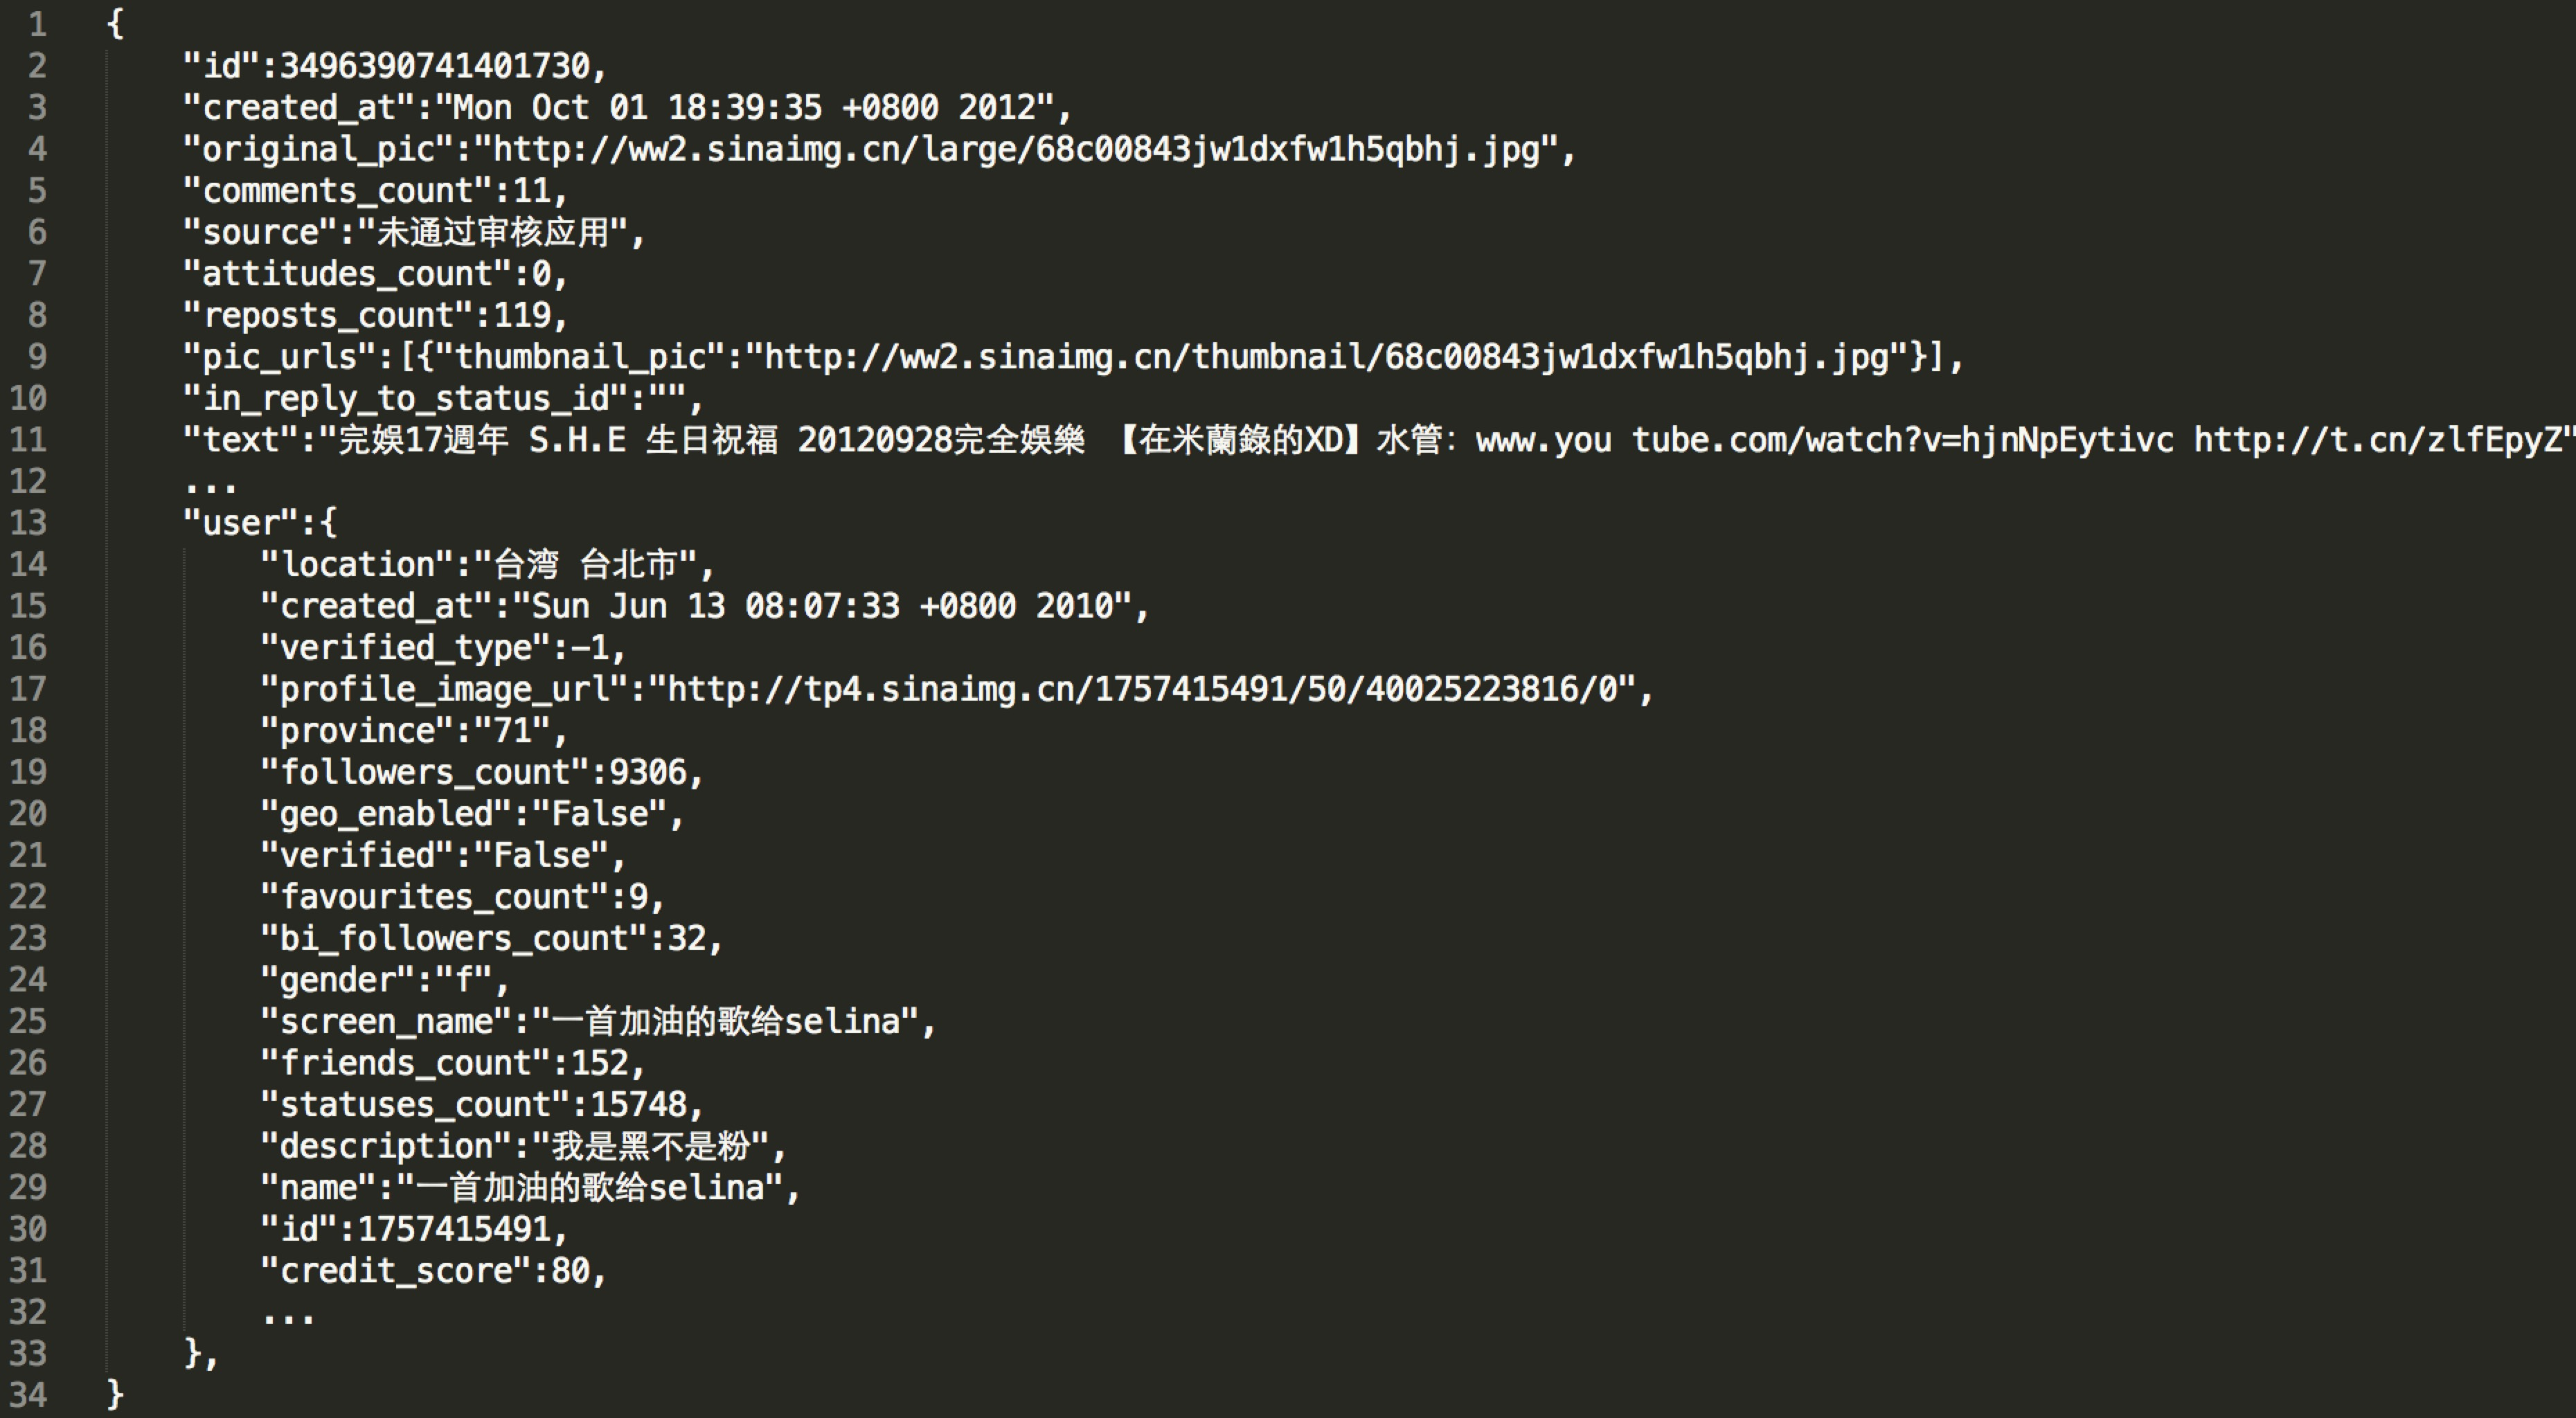
\includegraphics[width=1\textwidth]{JSON}
\caption{One sample crawled by Weibo API} \label{fig:JSON} 
\end{figure}

\section{Feature Extraction}
In Figure. \ref{fig:JSON} we can see the data are separated into two parts. From line 1 to line 12, those items are about the Weibo. For example, we can see the time of posting at line 3, the number of reposts at line 8, along with the text at line 11, so on and so forth. The rest of the content are about the author of this Weibo including the the number of posts at line 27 and friends count at line 28 and so on. Just for clarifying, in the user part, the \textit{created\_at} item represents the registered time of the user.

Then we introduce what feature we extract in this project. The feature we extract are mainly introduced by previous work. Experiments from related paper have shown that using those features can reach a good performance of model. We consider that those features are selected by domain knowledge\cite{yu2004incorporating}. However, the methods for extracting those features are not provided in their theses. Thus we try to use similar methods to extract them and we will discuss the methods in the next section. 

First we discuss the implicity features. After that, we integrate them with explicit features in a table.

\subsection{Implicity Feature}
Implicity Feature are mainly extracted from the Weibo text. We have extracted four types of features from the text.
\subsubsection{Emotion mark}
Chinese text is different from English because there is no space between each character. However, to analyze the emotion of the text, sentimental words is necessary. Thus we first need to split the sentence into several words. To do so, we use a third-party library called \textit{Jieba}\footnote{\url{https://github.com/fxsjy/jieba}} written in Python. Three types of cutting word mode are provided. We find the ``accurate mode'' are suitable for us. Besides, in order to remove some special charactors like ``[]'' or ``\#'', we use the regular expression to filter out them.

\begin{figure}[h]\centering 
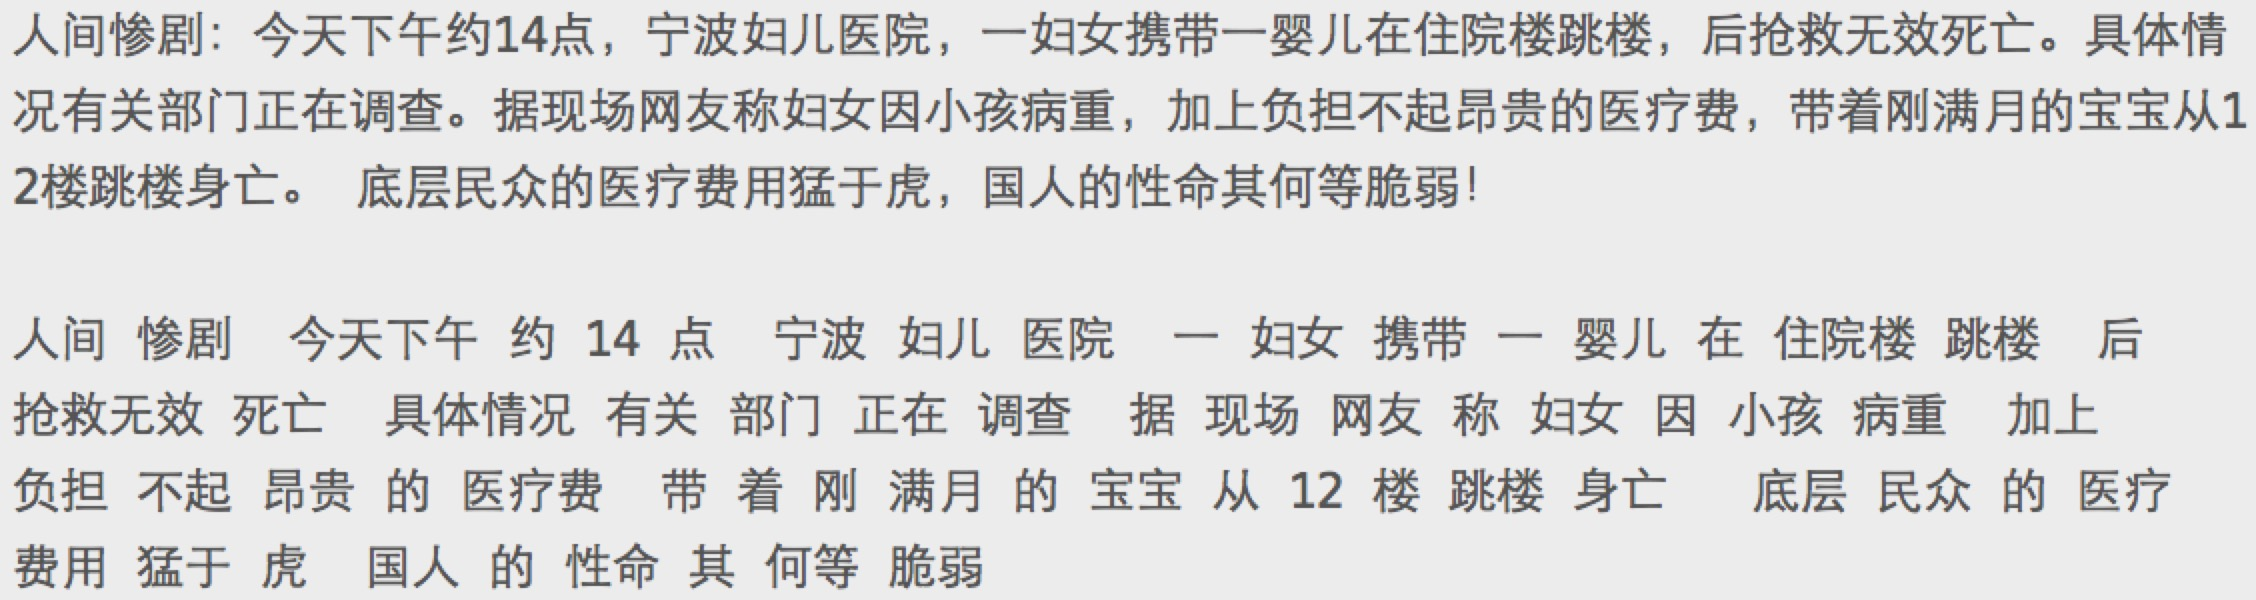
\includegraphics[width=1\textwidth]{splitword}
\caption{One Example of Word Split}\label{fig:WordSplit} 
\end{figure}

After we split the sentence into words, we need a dictionary containing emotional words to match. We use the dictionary provided by National Taiwan University called \textit{NTUSD}\footnote{\url{https://github.com/lackneets/NewsEvents/tree/master/lib/ntusd}}. This dictionary collects 2800 positive words and 8200 negative words. When we take the splitted sentence to match this dictionary, if the text contain a positive word, we give this text a +1 mark while -1 mark with negative word.

Meanwhile, user also may use emotion icon of emoji to express their feelings. For example, Weibo official emotion icon are represents in text as [good], [Weiwu] or [Nu]. User can also use apple emoji, such as \coloremoji{😂} or \coloremoji{😄}. We choose a part of them and manually classify the emotional direction. Identically, if the text has a icon or emoji which is classifying as a positive one, we give this text +1 mark. Otherwise -1 mark. We sum up all the marks this text acquires.

\subsubsection{Word Type}
Except for the sentimental analysis, we also propose a new set of features by calculating the percentage of the number of different type of word in the whole text, which are consisted of \textit{img}, \textit{real}, \textit{eng} and \textit{other}. Among, \textit{img} is the short for imaginary or function word and \textit{eng} is short for English word. The following table shows the rule of classifying which type each word is.
\begin{table}[!hbp] \centering
\begin{tabular}{|cIc|c|c|c|c|}
\hline
Real & adjective & verb & noun & numeral & pronoun\\
\hline
Img & exclamation & preposition & conjunction & auxiliary word & adverb\\
\hline
\end{tabular}
\caption{Word Type}
\end{table}

\subsubsection{Length}
The length of the text. Each word needs 3 bytes to store using utf-8 to encode.

\subsubsection{hasURL}
We use regular expression to match whether a text contain a url or not. 
This feature is an binary feature.
\begin{lstlisting}
http[s]?://(?:[\w\d]|[$-_@.&+]|(?:%[\w\d]))+
\end{lstlisting}

Along with the explicit feature, we extract 22 features as the vector to build our dataset in Table. \ref{Table:FeatureVector}

\begin{table}[h] \centering 
\begin{tabular}{lll}
\toprule
\textbf{Category} & \textbf{Feature} & \textbf{Description} \\
\midrule
\textbf{Text} & Emotion & The emotional mark of the text\\
& HasURL & Whether the message has URLs\\
& Length & The length of the message\\
& RealWord & The percentage of real word in the text\\
& ImgWord & The percentage of imaginary word in the text\\
& EngWord & The percentage of English word in the text\\
& OtherWord & The percentage of other word in the text\\
\textbf{User} & RegPostTime & Time span between registration and posting\\
& Verified & Whether the user is verified by Sina Weibo\\
& VerifiedType & Type of user based on verified information\\
& VerifiedKind & Similar to VerifiedType but more general\\
& Gender & Female or male\\
& GeoEnabled & Whether user enables the locating function\\
& Province & Where the user was registered\\
& FollowersCount & The number of people following this user\\
& FriendsCount & The number of people this user follows\\
& BiFollowersCount & The number of people mutually following\\
& StatusesCount & The number of status the user has posted\\
& FavouritesCount & The number of Weibo the user farourites\\
\textbf{Repost} & CommentCount & The number of comments the Weibo receives\\
& ShareCount & The number of repost from this Weibo\\
& AttributesCount & The number of like this Weibo receives\\
\bottomrule
\end{tabular}
\caption{Feature Vector and Description}
\label{Table:FeatureVector}
\end{table}



\section{Data Cleansing}
Data cleansing is a process of detecting illegal or inappropriate or missing data in the dataset and correcting them. It is an important part because incorrect data may lead to false conclusions. Sometimes, to let the algorithm can run smoothly without exception, missing value needs to be filled.

The methods of data cleansing is dependent on the specific application. Different types of error needs different methods. In our project, we are mainly facing the following types of errors.
\subsubsection{Negative value of \textit{time span}}
The value of this feature \textit{time span} is the span from the user registered time to the post time of that Weibo. The number of samples which have this type of error is small so that we can simply remove these samples.

\subsubsection{Number of \textit{BiFollowersCount $>$ FriendsCount}}
Mutual followers means two user follow each other. The number should be less or equal to the \textit{FriendsCount}. Thus we use the value of \textit{FriendsCount} as a substitute for the \textit{BiFollowersCount} dealing with this error.

\subsubsection{Value of \textit{StatusesCount} is 0}
Since we can crawl the Weibo of this user, thus its \textit{StatusesCount} can never be 0. Thus we simply set this feature as 1.


So far, the dataset has been built with roughly 4800 samples with 2400 rumor labeled as \textit{True} and 2400 not rumor labeled as \textit{False}. Fig. \ref{fig:finalDataset} is a part of our prepared dataset. In the next chapter, we want to introduce the theory of algorithms that can help us do analyzing the importance of the features.

\begin{figure}[h]\centering 
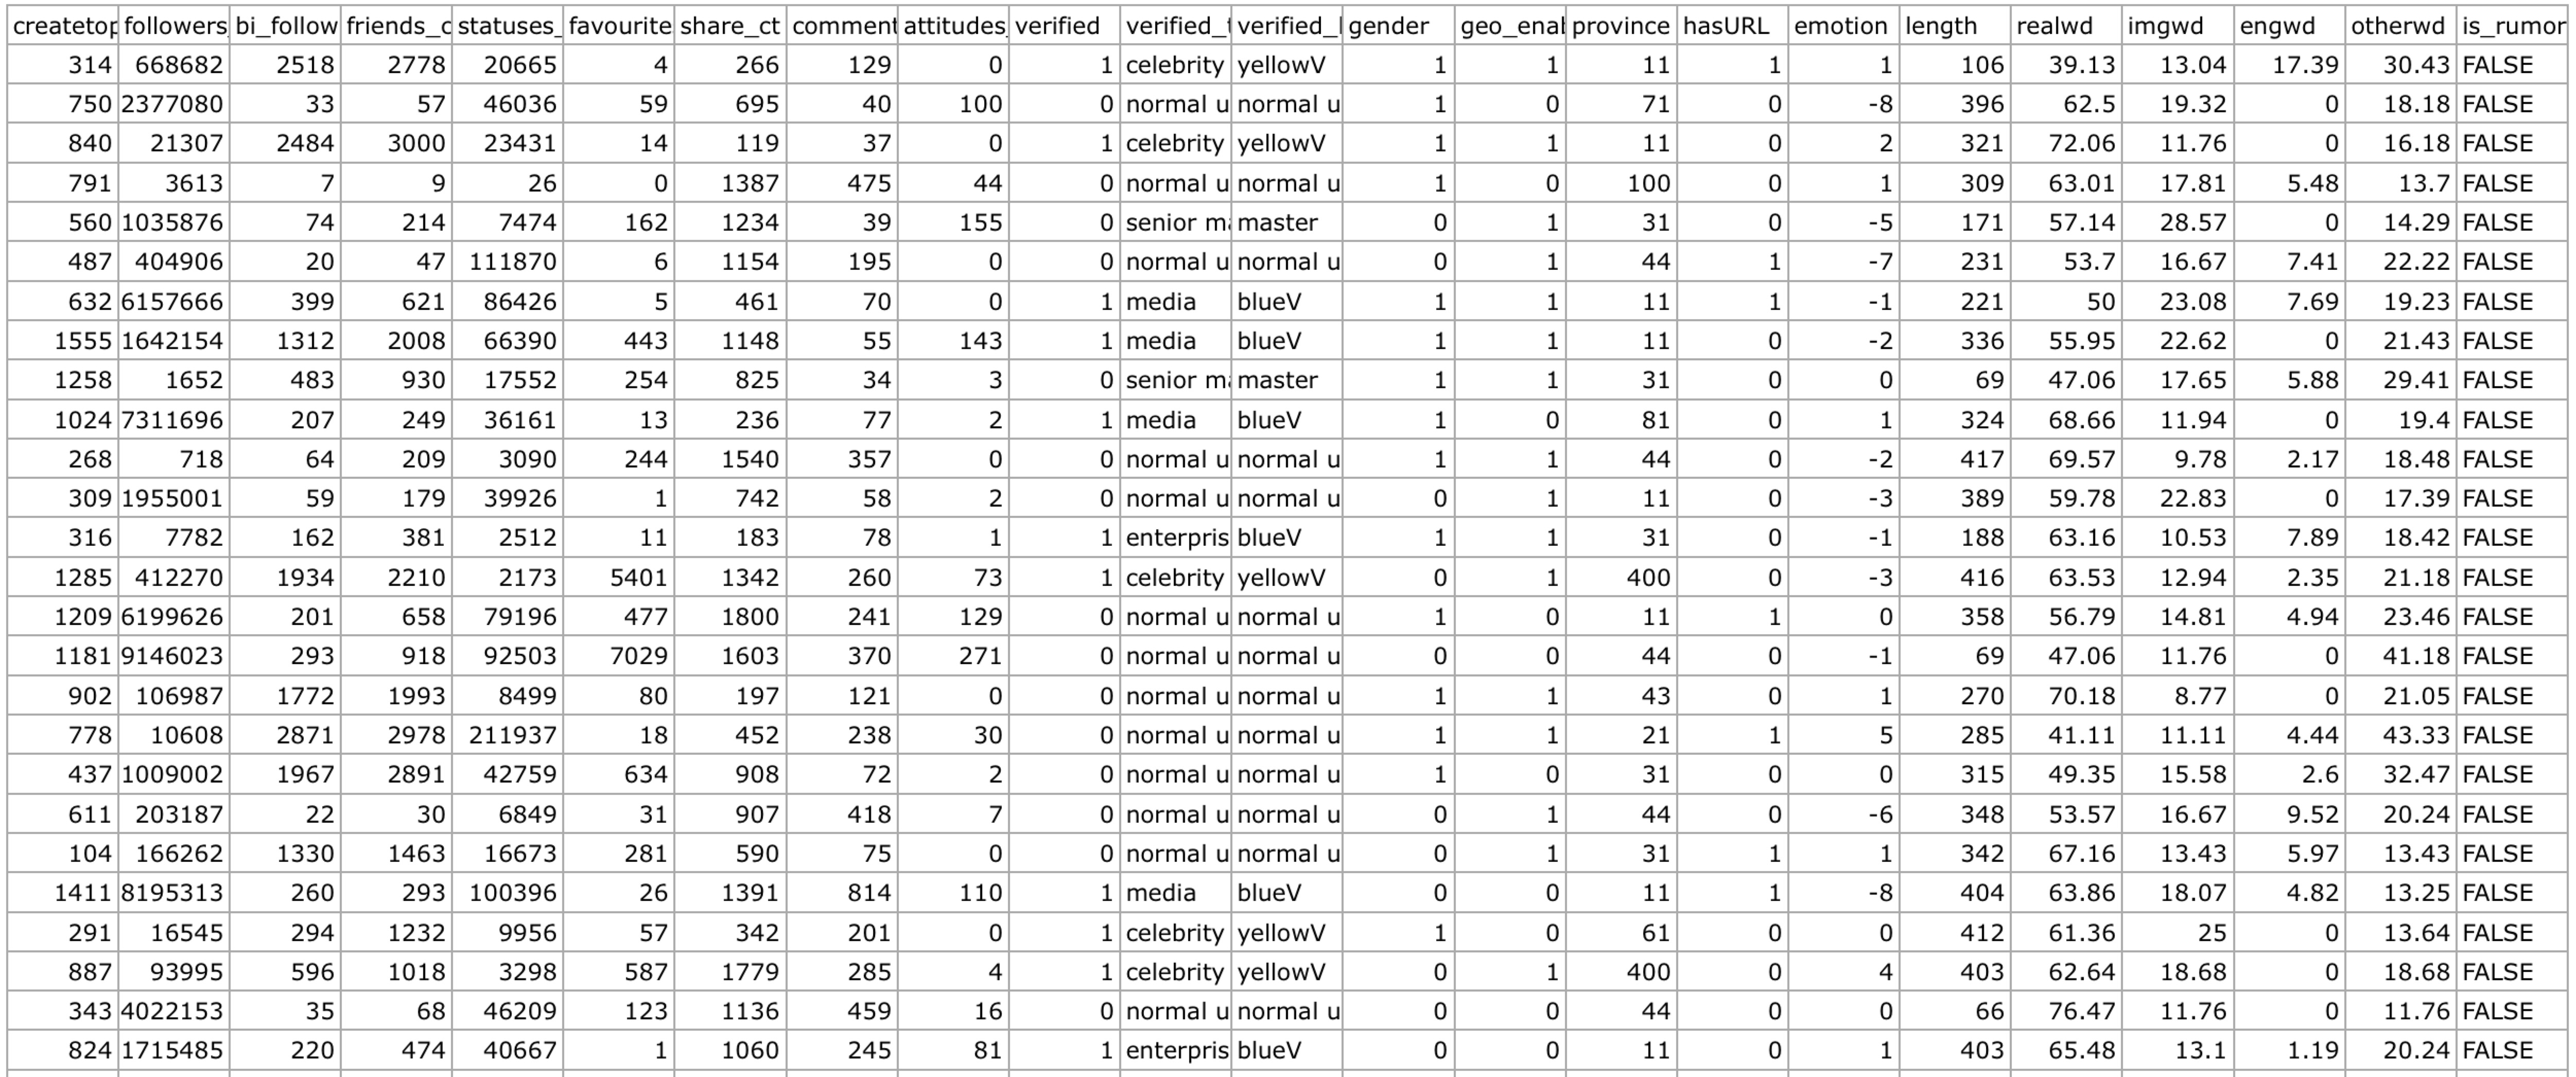
\includegraphics[width=1\textwidth]{finalDataset}
\caption{Extracted Dataset}\label{fig:finalDataset} 
\end{figure}






